
%% bare_conf.tex
%% V1.3
%% 2007/01/11
%% by Michael Shell
%% See:
%% http://www.michaelshell.org/
%% for current contact information.
%%
%% This is a skeleton file demonstrating the use of IEEEtran.cls
%% (requires IEEEtran.cls version 1.7 or later) with an IEEE conference paper.
%%
%% Support sites:
%% http://www.michaelshell.org/tex/ieeetran/
%% http://www.ctan.org/tex-archive/macros/latex/contrib/IEEEtran/
%% and
%% http://www.ieee.org/

%%*************************************************************************
%% Legal Notice:
%% This code is offered as-is without any warranty either expressed or
%% implied; without even the implied warranty of MERCHANTABILITY or
%% FITNESS FOR A PARTICULAR PURPOSE!
%% User assumes all risk.
%% In no event shall IEEE or any contributor to this code be liable for
%% any damages or losses, including, but not limited to, incidental,
%% consequential, or any other damages, resulting from the use or misuse
%% of any information contained here.
%%
%% All comments are the opinions of their respective authors and are not
%% necessarily endorsed by the IEEE.
%%
%% This work is distributed under the LaTeX Project Public License (LPPL)
%% ( http://www.latex-project.org/ ) version 1.3, and may be freely used,
%% distributed and modified. A copy of the LPPL, version 1.3, is included
%% in the base LaTeX documentation of all distributions of LaTeX released
%% 2003/12/01 or later.
%% Retain all contribution notices and credits.
%% ** Modified files should be clearly indicated as such, including  **
%% ** renaming them and changing author support contact information. **
%%
%% File list of work: IEEEtran.cls, IEEEtran_HOWTO.pdf, bare_adv.tex,
%%                    bare_conf.tex, bare_jrnl.tex, bare_jrnl_compsoc.tex
%%*************************************************************************

% *** Authors should verify (and, if needed, correct) their LaTeX system  ***
% *** with the testflow diagnostic prior to trusting their LaTeX platform ***
% *** with production work. IEEE's font choices can trigger bugs that do  ***
% *** not appear when using other class files.                            ***
% The testflow support page is at:
% http://www.michaelshell.org/tex/testflow/



% Note that the a4paper option is mainly intended so that authors in
% countries using A4 can easily print to A4 and see how their papers will
% look in print - the typesetting of the document will not typically be
% affected with changes in paper size (but the bottom and side margins will).
% Use the testflow package mentioned above to verify correct handling of
% both paper sizes by the user's LaTeX system.
%
% Also note that the "draftcls" or "draftclsnofoot", not "draft", option
% should be used if it is desired that the figures are to be displayed in
% draft mode.
%
\documentclass[conference]{IEEEtran}
% Add the compsoc option for Computer Society conferences.
%
% If IEEEtran.cls has not been installed into the LaTeX system files,
% manually specify the path to it like:
% \documentclass[conference]{../sty/IEEEtran}

\IEEEoverridecommandlockouts

% Turkce karakterler icin.
%\usepackage[turkish]{babel}
\usepackage[utf8]{inputenc}
\usepackage[T1]{fontenc}



% Some very useful LaTeX packages include:
% (uncomment the ones you want to load)


% *** MISC UTILITY PACKAGES ***
%
%\usepackage{ifpdf}
% Heiko Oberdiek's ifpdf.sty is very useful if you need conditional
% compilation based on whether the output is pdf or dvi.
% usage:
% \ifpdf
%   % pdf code
% \else
%   % dvi code
% \fi
% The latest version of ifpdf.sty can be obtained from:
% http://www.ctan.org/tex-archive/macros/latex/contrib/oberdiek/
% Also, note that IEEEtran.cls V1.7 and later provides a builtin
% \ifCLASSINFOpdf conditional that works the same way.
% When switching from latex to pdflatex and vice-versa, the compiler may
% have to be run twice to clear warning/error messages.






% *** CITATION PACKAGES ***
%
\usepackage{cite}
% cite.sty was written by Donald Arseneau
% V1.6 and later of IEEEtran pre-defines the format of the cite.sty package
% \cite{} output to follow that of IEEE. Loading the cite package will
% result in citation numbers being automatically sorted and properly
% "compressed/ranged". e.g., [1], [9], [2], [7], [5], [6] without using
% cite.sty will become [1], [2], [5]--[7], [9] using cite.sty. cite.sty's
% \cite will automatically add leading space, if needed. Use cite.sty's
% noadjust option (cite.sty V3.8 and later) if you want to turn this off.
% cite.sty is already installed on most LaTeX systems. Be sure and use
% version 4.0 (2003-05-27) and later if using hyperref.sty. cite.sty does
% not currently provide for hyperlinked citations.
% The latest version can be obtained at:
% http://www.ctan.org/tex-archive/macros/latex/contrib/cite/
% The documentation is contained in the cite.sty file itself.






% *** GRAPHICS RELATED PACKAGES ***
%
\ifCLASSINFOpdf
  \usepackage[pdftex]{graphicx}
  % declare the path(s) where your graphic files are
  % \graphicspath{{../pdf/}{../jpeg/}}
  % and their extensions so you won't have to specify these with
  % every instance of \includegraphics
  % \DeclareGraphicsExtensions{.pdf,.jpeg,.png}
\else
  % or other class option (dvipsone, dvipdf, if not using dvips). graphicx
  % will default to the driver specified in the system graphics.cfg if no
  % driver is specified.
  % \usepackage[dvips]{graphicx}
  % declare the path(s) where your graphic files are
  % \graphicspath{{../eps/}}
  % and their extensions so you won't have to specify these with
  % every instance of \includegraphics
  % \DeclareGraphicsExtensions{.eps}
\fi
% graphicx was written by David Carlisle and Sebastian Rahtz. It is
% required if you want graphics, photos, etc. graphicx.sty is already
% installed on most LaTeX systems. The latest version and documentation can
% be obtained at:
% http://www.ctan.org/tex-archive/macros/latex/required/graphics/
% Another good source of documentation is "Using Imported Graphics in
% LaTeX2e" by Keith Reckdahl which can be found as epslatex.ps or
% epslatex.pdf at: http://www.ctan.org/tex-archive/info/
%
% latex, and pdflatex in dvi mode, support graphics in encapsulated
% postscript (.eps) format. pdflatex in pdf mode supports graphics
% in .pdf, .jpeg, .png and .mps (metapost) formats. Users should ensure
% that all non-photo figures use a vector format (.eps, .pdf, .mps) and
% not a bitmapped formats (.jpeg, .png). IEEE frowns on bitmapped formats
% which can result in "jaggedy"/blurry rendering of lines and letters as
% well as large increases in file sizes.
%
% You can find documentation about the pdfTeX application at:
% http://www.tug.org/applications/pdftex





% *** MATH PACKAGES ***
%
\usepackage[cmex10]{amsmath}
% A popular package from the American Mathematical Society that provides
% many useful and powerful commands for dealing with mathematics. If using
% it, be sure to load this package with the cmex10 option to ensure that
% only type 1 fonts will utilized at all point sizes. Without this option,
% it is possible that some math symbols, particularly those within
% footnotes, will be rendered in bitmap form which will result in a
% document that can not be IEEE Xplore compliant!
%
% Also, note that the amsmath package sets \interdisplaylinepenalty to 10000
% thus preventing page breaks from occurring within multiline equations. Use:
%\interdisplaylinepenalty=2500
% after loading amsmath to restore such page breaks as IEEEtran.cls normally
% does. amsmath.sty is already installed on most LaTeX systems. The latest
% version and documentation can be obtained at:
% http://www.ctan.org/tex-archive/macros/latex/required/amslatex/math/





% *** SPECIALIZED LIST PACKAGES ***
%
%\usepackage{algorithmic}
% algorithmic.sty was written by Peter Williams and Rogerio Brito.
% This package provides an algorithmic environment fo describing algorithms.
% You can use the algorithmic environment in-text or within a figure
% environment to provide for a floating algorithm. Do NOT use the algorithm
% floating environment provided by algorithm.sty (by the same authors) or
% algorithm2e.sty (by Christophe Fiorio) as IEEE does not use dedicated
% algorithm float types and packages that provide these will not provide
% correct IEEE style captions. The latest version and documentation of
% algorithmic.sty can be obtained at:
% http://www.ctan.org/tex-archive/macros/latex/contrib/algorithms/
% There is also a support site at:
% http://algorithms.berlios.de/index.html
% Also of interest may be the (relatively newer and more customizable)
% algorithmicx.sty package by Szasz Janos:
% http://www.ctan.org/tex-archive/macros/latex/contrib/algorithmicx/




% *** ALIGNMENT PACKAGES ***
%
%\usepackage{array}
% Frank Mittelbach's and David Carlisle's array.sty patches and improves
% the standard LaTeX2e array and tabular environments to provide better
% appearance and additional user controls. As the default LaTeX2e table
% generation code is lacking to the point of almost being broken with
% respect to the quality of the end results, all users are strongly
% advised to use an enhanced (at the very least that provided by array.sty)
% set of table tools. array.sty is already installed on most systems. The
% latest version and documentation can be obtained at:
% http://www.ctan.org/tex-archive/macros/latex/required/tools/


%\usepackage{mdwmath}
%\usepackage{mdwtab}
% Also highly recommended is Mark Wooding's extremely powerful MDW tools,
% especially mdwmath.sty and mdwtab.sty which are used to format equations
% and tables, respectively. The MDWtools set is already installed on most
% LaTeX systems. The lastest version and documentation is available at:
% http://www.ctan.org/tex-archive/macros/latex/contrib/mdwtools/


% IEEEtran contains the IEEEeqnarray family of commands that can be used to
% generate multiline equations as well as matrices, tables, etc., of high
% quality.


%\usepackage{eqparbox}
% Also of notable interest is Scott Pakin's eqparbox package for creating
% (automatically sized) equal width boxes - aka "natural width parboxes".
% Available at:
% http://www.ctan.org/tex-archive/macros/latex/contrib/eqparbox/





% *** SUBFIGURE PACKAGES ***
%\usepackage[tight,footnotesize]{subfigure}
% subfigure.sty was written by Steven Douglas Cochran. This package makes it
% easy to put subfigures in your figures. e.g., "Figure 1a and 1b". For IEEE
% work, it is a good idea to load it with the tight package option to reduce
% the amount of white space around the subfigures. subfigure.sty is already
% installed on most LaTeX systems. The latest version and documentation can
% be obtained at:
% http://www.ctan.org/tex-archive/obsolete/macros/latex/contrib/subfigure/
% subfigure.sty has been superceeded by subfig.sty.



%\usepackage[caption=false]{caption}
%\usepackage[font=footnotesize]{subfig}
% subfig.sty, also written by Steven Douglas Cochran, is the modern
% replacement for subfigure.sty. However, subfig.sty requires and
% automatically loads Axel Sommerfeldt's caption.sty which will override
% IEEEtran.cls handling of captions and this will result in nonIEEE style
% figure/table captions. To prevent this problem, be sure and preload
% caption.sty with its "caption=false" package option. This is will preserve
% IEEEtran.cls handing of captions. Version 1.3 (2005/06/28) and later
% (recommended due to many improvements over 1.2) of subfig.sty supports
% the caption=false option directly:
%\usepackage[caption=false,font=footnotesize]{subfig}
%
% The latest version and documentation can be obtained at:
% http://www.ctan.org/tex-archive/macros/latex/contrib/subfig/
% The latest version and documentation of caption.sty can be obtained at:
% http://www.ctan.org/tex-archive/macros/latex/contrib/caption/




% *** FLOAT PACKAGES ***
%
%\usepackage{fixltx2e}
% fixltx2e, the successor to the earlier fix2col.sty, was written by
% Frank Mittelbach and David Carlisle. This package corrects a few problems
% in the LaTeX2e kernel, the most notable of which is that in current
% LaTeX2e releases, the ordering of single and double column floats is not
% guaranteed to be preserved. Thus, an unpatched LaTeX2e can allow a
% single column figure to be placed prior to an earlier double column
% figure. The latest version and documentation can be found at:
% http://www.ctan.org/tex-archive/macros/latex/base/



%\usepackage{stfloats}
% stfloats.sty was written by Sigitas Tolusis. This package gives LaTeX2e
% the ability to do double column floats at the bottom of the page as well
% as the top. (e.g., "\begin{figure*}[!b]" is not normally possible in
% LaTeX2e). It also provides a command:
%\fnbelowfloat
% to enable the placement of footnotes below bottom floats (the standard
% LaTeX2e kernel puts them above bottom floats). This is an invasive package
% which rewrites many portions of the LaTeX2e float routines. It may not work
% with other packages that modify the LaTeX2e float routines. The latest
% version and documentation can be obtained at:
% http://www.ctan.org/tex-archive/macros/latex/contrib/sttools/
% Documentation is contained in the stfloats.sty comments as well as in the
% presfull.pdf file. Do not use the stfloats baselinefloat ability as IEEE
% does not allow \baselineskip to stretch. Authors submitting work to the
% IEEE should note that IEEE rarely uses double column equations and
% that authors should try to avoid such use. Do not be tempted to use the
% cuted.sty or midfloat.sty packages (also by Sigitas Tolusis) as IEEE does
% not format its papers in such ways.





% *** PDF, URL AND HYPERLINK PACKAGES ***
%
%\usepackage{url}
% url.sty was written by Donald Arseneau. It provides better support for
% handling and breaking URLs. url.sty is already installed on most LaTeX
% systems. The latest version can be obtained at:
% http://www.ctan.org/tex-archive/macros/latex/contrib/misc/
% Read the url.sty source comments for usage information. Basically,
% \url{my_url_here}.

% *** Do not adjust lengths that control margins, column widths, etc. ***
% *** Do not use packages that alter fonts (such as pslatex).         ***
% There should be no need to do such things with IEEEtran.cls V1.6 and later.
% (Unless specifically asked to do so by the journal or conference you plan
% to submit to, of course. )

\usepackage{multirow}
\usepackage{array}
\usepackage[lofdepth,lotdepth]{subfig}
\hyphenation{op-tical net-works semi-conduc-tor}


\begin{document}

%\IEEEpubid{\makebox[\columnwidth]{978-1-4799-4874-1/14/\$31.00 ©2015 IEEE\hfill}https://tr.overleaf.com/project/6005dff19b5222b1edc6102a
%\hspace{\columnsep}\makebox[\columnwidth]{}}

%
% paper title
% can use linebreaks \\ within to get better formatting as desired
\title{Pulumi Bulut Yazılımı Oluşturma Aracı}
\author{\IEEEauthorblockN{Seher Aydın,162805011}
\IEEEauthorblockA{Yazılım Mühendisliği Bölümü\\
Celal Bayar Üniversitesi\\
Manisa, Türkiye\\
\ }
}

\maketitle
\begin{ozet}
Bu çalışmada C\# dili ile hazırlanmış bir bulut yazılımı oluşturma aracının 9 versiyonu incelenmiştir. Açık kaynak kodlu bir yazılımdır. Gelişimi hala devam etmektedir. İncelenen versiyonlar için Chidember-Kemerer MetricSet, diğer metrikler ile QMOOD Modeli kullanılarak tasarım kalitesi nitelikleriyle ilgili sayısal ölçümler elde edilmiştir. Uygulamada yapılan versiyon güncellenmeleriyle ilgili nitreliklerin değişimi incelenilerek elde edilen sonuçlar değerlendirilmiştir. 
\end{ozet}
\begin{IEEEanahtar}
Nesneye Dayalı Programlama, QMOOD, OOP, Tasarım Kalitesi Nitelikleri, NDepended
\end{IEEEanahtar}
\begin{abstract}
In this work, nine versions of a  application  is implemented by C# programming language is studied. Chidember-Kemerer MetricSet and QMOOD Model is used for the investigation between application versions. Considering different versions of the application, the change of computed quality attributes are evaluated
\end{abstract}
\begin{IEEEkeywords}
Quality attributes, Object Oriented Programming, QMOOD
\end{IEEEkeywords}
\IEEEpeerreviewmaketitle

\IEEEpubidadjcol


\section{GİRİŞ}

Yazılım teknolojilerinin farklı alanlarda farklı görevlerde teknlojiye yönelik bir çok cihazda yaygın olarak kullanılmaya başlanması, kullanılan yazılımların değerlendirilerek geri besleme yapılması ihtiyacını doğurmuştur. Yazılım  kalitesinin gözlemlenerek, aynı işlevi yerine getiren birden fazla yazılımdan hangisinin daha iyi olduğunu söylemek mümkün değildir. Yazılım kalitesinin ölçülmesinde gerçek dünyada gözlem yapmayı olanaksız kılan bilgi engelinden dolayı karşılaştırmalar yapmak ve yorumlar ölçme yoluyla dolaylı olarak yapılmaktadır. Değerlendirme gözlem yoluyla gerçek dünyada dĕgil, ölçme  ile elde  edilen sayısal veri üzerinden yapılarak yorumlanabilir. Chidember-Kemerer  Metrik  Kümesinden \cite{label1}.\\  yararlanarak  ve nesneye dayalı tasarımlar için sezgisel dünya ile formel dünyaarasında  bir  model  sunan  QMOOD  Modeli,  temsilin doğruluğu  açısından başarıyla  sınanmı̧s  modellerden  biridir  \cite{label2}.
Bu bağlamda, bu çalışmada QMOOD Modeli kullanılarak Pulumi adlı yazılım, windows platform için C# programala dili kullanılarak hazırlanan bu uygulamanın V.1.0.0-V1.4.0 versiyon aralıklarını kalite niteliklerinin değişimi açısından incelenmiştir. Bu uygulama açık kaynak kodludur. Gelişimi hala devam etmektedir.


\section{İncelenen Yazılım}
Pulumi'nin Kod SDK Olarak Altyapısı , herhangi bir bulut üzerinde kapsayıcılar, sunucusuz işlevler, barındırılan hizmetler ve altyapı kullanan bulut yazılımı oluşturmanın ve dağıtmanın en kolay yoludur \cite{label3}.Biz bu sebeplerden dolayı pulumi inceledik bu yazılımın incelemesinde Visual Studio Community 16.8.3 ve ndepend Version v2020.2.1 araçlarını kullandık.

\section{İlgİlİ Çalışmalar}
Yazılım kalitesinin ölçülmesi konusunda son yıllarda literatürde bir çok çalı̧sma yer almaktadır\cite{label5},
\cite{label6},\cite{label7},\cite{label8}’da sezgisel dünya ile formel dünya arasındaki temsil için olu̧sturulan modeller incelenmiştir .Benzer şekilde [2]'de nesneye dayalı tasarım kalitesini dĕgerlendirmek amacıyla oluşturulan hiyerarşik model ele alınmıştır.\cite{label9}’daki çalı̧smada yer alan ve McCall tarafından oluşturulan yazılım modeli, yazılım paydaşları arasında iletişim sağlamayı amaçlamıştır ve pek çok yazılıma temel oluşturmaktadır.

\section{KULLANILAN YAKLAŞIM ve ARAÇLAR}\label{sec:uc}
QMOOD bir yazılım kalitesi inceleme modelidir. Modeller, bir yazılımın farklı parametrelerini degerlendirip sonucunda insan için anlamlı çıktılara ulaşmaya çalışırlar.Bu çıkarımlara ulaşmak adına QMOOD, yazılımın ham verilerininin(L4) yanısıra yazılım nitelikleri(L1), yazılım özellikleri(L2), yazılım metrikleri(L3) olarak düzeylendirilmiştir.QMOOD modeli temelinde bir yazılımın kalitesini 11 temel metrik ve bunların etkiledigi gözlemlenebilir 6 nitelikle inceler.QMOOD kapsamında kullanıcıya en çok hitap eden parçalar yazılım nitelikleridir. Bu nitelikler modelin daha küçük parçalardan ulaştıgı sonuçlardır Bu bölümde, kullanılan yaklaşım ve kullanılan araçlara yer vericeğiz.\\
\subsection{Kullanılan Yaklaşım}
Şu şekilde formülize edilirler ( L1 - L2 Geçicisi ) :
\begin{equation}
\textit{Tekrar Kullan{\i}labilirlik=}
\begin{cases}
+0,5\cdot(Desing~Size) &  \\
-0,25\cdot(Coupling) & \\
+0,25\cdot(Cohesion) &  \\
+0,5\cdot(Messaging)& \\
\end{cases}
\label{equ:reuse}
\end{equation}

\begin{equation}
\textit{Esnek{\i}lik=}
\begin{cases}
+0,25\cdot(Encapsulation) &  \\
-0,25\cdot(Coupling) & \\
+0,5\cdot(Composition) &  \\
+0,5\cdot(Polymorphsim)& \\
\end{cases}
\label{equ:reuse}
\end{equation}

\begin{equation}
\textit{Anlaşır{\i}lık=}
\begin{cases}
-0,33\cdot(Desing Size) &  \\
-0,33\cdot(Abstraction) & \\
+0,33\cdot(Encapsulation) &  \\
-0,33\cdot(Coupling) & \\
+0,33\cdot(Cohesion) & \\
-0,33\cdot(Polymorphsim)& \\
+0,33\cdot(Complexity) & \\
\end{cases}
\label{equ:reuse}
\end{equation}

\begin{equation}
\textit{İşlev{\i}sellik=}
\begin{cases}
+0,22\cdot(Design Size) &  \\
+0,22\cdot(Hierarchies)) & \\
+0,12\cdot(Cohesion) &  \\
+0,22\cdot(Polymorphsim)& \\
+0,12\cdot(messaging) &  \\
\end{cases}
\label{equ:reuse}
\end{equation}

\begin{equation}
\textit{Geniletil{\i}ebilirlik=}
\begin{cases}
+0,5\cdot(Abstraction) &  \\
-0,5\cdot(Coupling) & \\
+0,5\cdot(Inheritance)) &  \\
+0,5\cdot(Polymorphism)& \\
\end{cases}
\label{equ:reuse}
\end{equation}

\begin{equation}
\textit{Etkin{\i}lik=}
\begin{cases}
+0,20\cdot(Abstraction) &  \\
+0,20\cdot(Encapsulation)) & \\
+0,20\cdot(Composition) &  \\
+0,20\cdot(Inheritance)& \\
+0,20\cdot(Polymorphism) &  \\
\end{cases}
\label{equ:reuse}
\end{equation}

Yazılım nitelikleri ile yazılım özellikleri arasındaki ilişki,birçok özelliğin harmanlayıp bizlere daha özütülmüş bilgi vermeyi amaçlamaktadır Bir alt seviyeye inildiginde diger bir düzey olan yazılım metrikleri bizi karsılamaktadır. Yazılım metrikleri, temel anlamda kodun daha somut ve sayılabilir verilerini (Satır Sayısı,Sınıf Sayısı, Kod satırı Sayısı gibi. ) matematiksel hesaplamalar veya gösterimler adına daha kolay işlenebilir hale getirmektedir.

\begin{table}[h]
	\centering
	\begin{tabular}{|c|c|}
		\hline
		\textbf{Tasarım Özelliği}	& \textbf{İlgili Tasarım Metriği}\\
		\hline
		Design Size	& Design Size in Classes\\
		\hline
		Complexity & Number of Methods\\
		\hline
		Hierarchies & Number Hierarchies (NOH)\\
		\hline
		Messaging & Class  Interface Size (CIS)\\
		\hline
		Composition & Measure  Aggregation (MOA)\\
		\hline
		Encapsulation & Data Access Metric (DAM)\\
		\hline
		Coupling & Direct Class Coupling (DCC)\\
		\hline
		Inheritance & Measures of Functional Abstraction (MFA)\\
		\hline
		Polymorphism & Number of Polymorphic Methods (NOP)\\
		\hline
		Cohesion & Cohesion Among Methods (CAM)\\
		\hline
		Abstraction & Average Number of Ancestors (ANA)\\
		\hline


		
	\end{tabular}
	\caption{Tasarım Metrikleri ile Tasarım Özellikleri Arasındaki İlişki}
	\label{table:1}
\end{table}
Örnek bir item list:

\begin{itemize}
	\item \textbf{Design Size in Classes (DSC):} Projedeki toplam sınıf sayısı olarak değerlendirilmiştir.
	\item \textbf{Number of Hierarchies (NOH):} Projedeki sınıf hiyararşi sayısı olarak ele alınmıştır.
	\item \textbf{Average Number of Ancestors (ANA):} Projedeki kalıtım ağacı boyunun ortalaması olarak hesaplanmıştır.
	\item \textbf{Class Interface Size (CIS):} Sınıfın açık (public)
metotlarının sayısıdır ve yazılımın mesajlaşma özelliği
hakkında fikir verir.

	\item \textbf{Measure Of Aggregation (MOA) :}  Kullanıcı tarafından tanımlanmı¸s sınıfların temel sistem veri tiplerine
(int, char, double vs. . . ) oranıdır.

	\item \textbf{Data Access Metric (DAM) :}  : Sınıfın özel(private)
ve korumalı(protected) niteliklerinin tüm niteliklere
oranıdır.

	\item \textbf{Cohesion Among Methods (CAM) :}  Metotların
imzaları arasındaki benzerligin ölçüsüdür.
	\item \textbf{Direct Class Coupling (DCC) :} : Birbiriyle doğrudan 
ilişkili olan sınıfların sayısıdır.
	\item \textbf{Inheritance (MFA):}  : Sınıfın kalıtımla aldıgı metot 
sayısının kendi barındırdığı metot sayısı oranıdır.
	\item \textbf{Number of Polymorphism (NOP) :}  Kalıtılan toplam
metot sayısıdır.

	\item \textbf{• Number of Methods (NOM) :}  Sınıfın metot sayısıdır.
\end{itemize}



\subsection{Kullanılan Araçlar}
\textbf{• Ndepend ve Visual Studio Community :} Bir visual Studio eklentisi olan ndepend ile c\# projeleri  metrikleri teste tabii tutulabilmektedir. \cite{label4}. Visual Studio Community ise Visual Studio içerisinden halii hazırda erişilebilir bir araçtır.

\begin{figure}[h]
	\centering
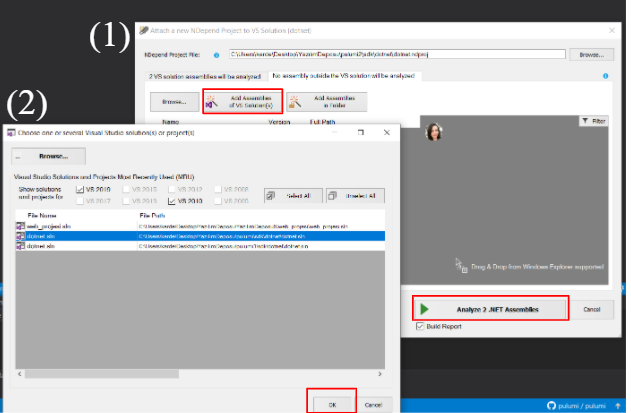
\includegraphics[scale=0.785]{3.png}
	\caption{Ndepend Eklentisi ile Metrik Çıkarımı}
	\label{sekil1}
\end{figure}

\begin{figure}[h]
	\centering
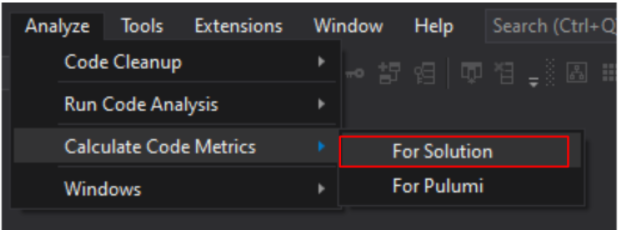
\includegraphics[scale=0.550]{VS Community.png}
	\caption{Visual Studio Community Eklentisi ile Metrik Çıkarımı}
	\label{sekil2}
	

\end{figure}





\vspace{150}
\section{DEĞERLENDİRME}
\subsection{Tasarım Niteliklerinin Bulunması}
İncelediğimiz projenin tasarım niteliklerini yalın bir şekilde
 açıklayabilmek için niteliklerin sınıflara göre ağırlıklı 
ortalamasını alıp daha sonrasında bu değerleri belli bir sayı 
aralığına indirgemek için de bu niteliklerin standart sapmalarını 
hesaplayıp sonrasında grafiğe aktarma yoluna gittik.

Yukarıda resimlerde gördüğünüz üzere ndepend eklentisi ile visual studio içerisinde hem visual studio'nun vermiş olduğu eklentiler kullanılarak hemde ndepend eklentisi aracılığı ile  açık kaynak kodlu yazılımın metrik değerleri çıkarılabilmektedir.
Grafikte kullandığımız değerler aşağıda verilmiştir;

\begin{table*}
\begin{tabular}{|c|c|c|c|c|c|c|c|c|c|c|c|}
\hline
\textbf{Versiyon} & \textbf{Encapsulation} & \textbf{Polymorfism} & \textbf{Hieracies} & \textbf{Messaging} & \textbf{Design Size} & \textbf{Composotion} & \textbf{Abstract} & \textbf{Inheritance} & \textbf{Cohesion} & \textbf{Complexity} & \textbf{Coupling} \\ \hline
V.1.0.0           & 1                      & 1                    & 1                  & 1                  & 1                    & 1                    & 1                 & 1                    & 1                 & 1                   & 1                 \\ \hline
V.1.10            & 1,75                   & 0,73                 & 1,75               & 1                  & 0,23                 & 1                    & 1,75              & 0,18                 & 0,75              & 1,02                & 1,08              \\ \hline
V.1.2.0           & 1                      & 0,73                 & 1                  & 1                  & 0,23                 & 1,03                 & 0,55              & 0,4                  & 0,75              & 0,99                & 1                 \\ \hline
V.1.3.0           & 1                      & 1                    & 1                  & 0,96               & 0,27                 & 0,95                 & 0,12              & 0,18                 & 0.5               & 0,99                & 1                 \\ \hline
V.1.3.1           & 1                      & 0,77                 & 1                  & 1,07               & 0,25                 & 1,02                 & 0,09              & 0,55                 & 1,5               & 0,98                & 1                 \\ \hline
V.1.3.2           & 1                      & 0,83                 & 1                  & 0,95               & 0,24                 & 1,06                 & 0,11              & 0,55                 & 1.25              & 0,95                & 1                 \\ \hline
V.1.3.3           & 1                      & 0,88                 & 1                  & 1,05               & 0,25                 & 1                    & 0,14              & 0,18                 & 1,5               & 0,99                & 1                 \\ \hline
V.1.3.4           & 1                      & 0,82                 & 1                  & 0,96               & 0,21                 & 1,03                 & 0,21              & 0,18                 & 1,25              & 1                   & 1                 \\ \hline
V.1.4.0           & 1                      & 0,83                 & 1                  & 0,98               & 0,21                 & 1,02                 & 0,2               & 0,55                 & 1                 & 0,99                & 1                 \\ \hline
\end{tabular}
\end{table*}

\begin{table*}
\begin{tabular}{|c|c|c|c|c|c|c|}
\hline
\textbf{Versiyon} & \textbf{Tekrar Kullanılabilirlik} & \textbf{Esneklik} & \textbf{İşlevsellik} & \textbf{Genişletilebilirlik} & \textbf{Etkinlik} & \textbf{Anlaşılabilirlik} \\ \hline
V.1.0.0           & 1                                 & 1                 & 1                    & 1                            & 1                 & -1                        \\ \hline
V.1.10            & 0,5325                            & 1,0325            & 0,9956               & 1                            & 1                 & -0,99                     \\ \hline
V.1.2.0           & 0,5525                            & 0,88              & 0,7412               & 0,79                         & 1,082             & -0,7623                   \\ \hline
V.1.3.0           & 0,49                              & 0,975             & 0,75                 & 0,34                         & 0,742             & -0,5775                   \\ \hline
V.1.3.1           & 0,785                             & 0,895             & 0,7662               & 0,15                         & 0,65              & -0,6204                   \\ \hline
V.1.3.2           & 0,6575                            & 0,945             & 0,8576               & 0,205                        & 0,686             & -0,1947                   \\ \hline
V.1.3.3           & 0,775                             & 0,94              & 0,8166               & 0,245                        & 0,71              & -0,2904                   \\ \hline
V.1.3.4           & 0,6475                            & 0,925             & 0,8708               & 0,1                          & 0,64              & -0,2508                   \\ \hline
V.1.4.0           & 0,605                             & 0,925             & 0,8122               & 0,105                        & 0,648             & -0,3267                   \\ \hline
\end{tabular}
\end{table*}

Projede bulunan 9 farklı versiyon için farklı metrik değerleri gerek hem visual studio gerekse ndepend eklentisi aracılığı ile teste tabii tuttuğumuzda çıkan  sonuçları normalizasyon işleminden geçirdikten sonra exel aracılığa ile grafiğe döktüğümüz zaman elimizde aşağıda gözüken tarzda tablolar ortaya çıkmıştır.

\begin{figure}[h]
	\centering
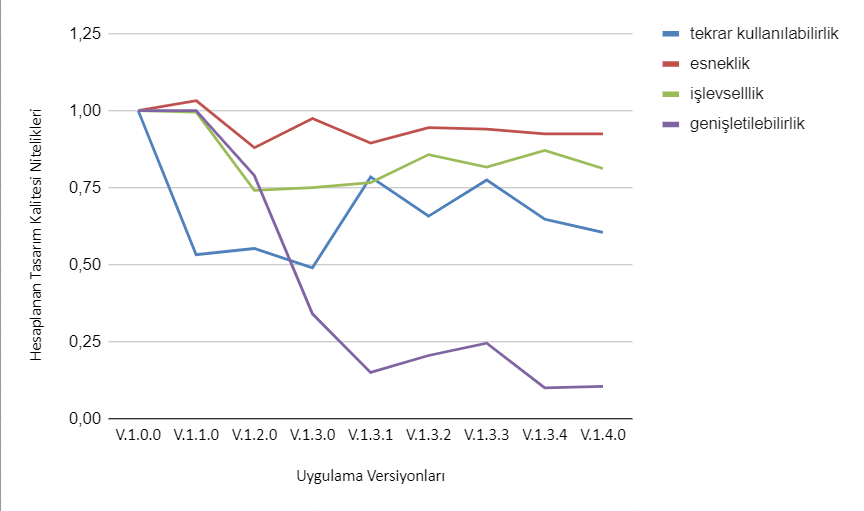
\includegraphics[scale=0.515]{grafik1.png}
	\caption{Farklı Versiyonlar için Etkinlik, Genişletilebilirlik, İşlevsellik,Tekrar kullanılabilirlik ve Esneklik Niteliklerinin değişimi}
	\label{Grafik1}
\end{figure}


Farklı Versiyonlar için 
  
\begin{itemize}
\item   Etkinlik, 
\item    Genişletilebilirlik, 
\item    İşlevsellik,
\item    Tekrar kullanılabilirlik 
\item    Esneklik 
\end{itemize}

Niteliklerinin  9 farklı versiyon için  bu metriklerin versiyona bağlı olarak değişimi yukarıda gösterilmiştir. Bu hesaplamalarda yer alan niteliklere özgü sayısal veriler y ekseninde yer alırken versiyonun numaraları ise en altta x ekseni düzleminde yer almaktadır.Sezgisel olarak baktığımızda ise bu  sayısal verilerin en başta artarak yükselmesi beklenmektedir fakat esneklik en başta ufak miktar artmış olsa bile sonradan düşüşe geçmiş ve geri kalan tüm veriler aşağı  ve yukarı şeklinde ilerlemelerine rağmen genel yönelim aşağı yöne doğru olmuştur. Bu  beklenmedik düşüşün sebebi uygulamanın ilk versiyonun yeterince nesneyeli yönelik olmaması , clean code şeklinde yazılmaması ve tekrarlanan fonksiyon ve benzeri öğelerin düzenlenmemesi ilk başta karışık bir versiyon ile çıktıktan sonra diğer versiyonlarda bu durumun iyileştirilmesi şeklinde yorumlanabilir.

Aşağıda farklı Versiyonlar için 
\begin{itemize}
\item Anlaşılabilirlik
\end{itemize}
Niteliğinin  9 farklı versiyon için  bu metriklerin versiyona bağlı olarak değişimi yukarıda gösterilmiştir. Bu hesaplamalarda yer alan niteliklere özgü sayısal veriler y ekseninde yer alırken versiyonun numaraları ise en altta x ekseni düzleminde yer almaktadır. Sezgisel olarak bakıldığında anlaşılabilirlik metriğinin ilk başta azalması sonra artması beklenmektedir fakat  ilk grafiktede yaşanan bu beklenmedik durum burada da yaşanarak tahminlerimizin doğuluğunu göstermektedir. Anlaşılabilirlik ilk başta projenin karmşıklığı sebebi ile düşük olsada sonradan bu değerler yukarı yönlü bir ivme göstermiştir.  V1.3.0-V1.3.2-V1.3.4 te ufak düşüşler yaşasada genel olarak yükselmiştir.
\begin{figure}[h]
	\centering
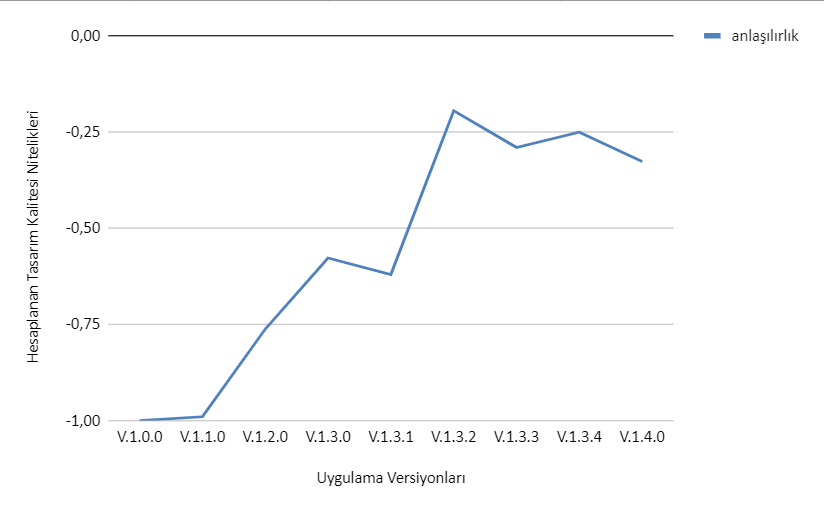
\includegraphics[scale=0.515]{grafik2.png}
	\caption{Farklı Versiyonlar için Anlaşılabilirlik Niteliğinin Değişimi}
	\label{Grafik2}
\end{figure}

\vspace{500}
\section{SONUÇ}

Bu çalışmada windows platform için c\# programala dili kullanılarak hazırlanan bir mobil uygulama ele alınmıştır. Bu uygulamanın  1 yıl içerisinde geliştirilip açık kaynak kodlu olarak yayınlanan 9 farklı versiyonu  QMOOOD modeli kullanılarak incelenmiştir. Sonuç olarak değerlendirdiğimizde ise ilgili modelin kullanılan yaklaşımın sezgisel olarak beklenen değerlerden farklı bir çıktı verdiği fakat kendi içinde tutarlı olduğu gözlemlenmiştir. Tasarımın bir uygulama içerisinde ki değişimi nesneye yönelik  dayalı tasarım kriterleri göz önüne alınarak hazırlanan uygulamanın doğruluğunu göstermiştir. Ayrıca çıkan kalite niteliklerinin değişim karakteristiğine bakıldığı zaman projenin geliştirilmesi sırasında yapılan hata düzeltme ve projeyi düzeltme esnasında yapılan sürümler güncellemelerinde nesneye dayalı programlamaa presinsiplerinden uzaklaşdığı yada dikkate alınmadığı söylenebilir. Esas geliştirme sonrasında projenin büyük çoğunlunun düzeltme ve onarma işlemi ile geçtiğini de vurgulanabilir. Proje ile ilgili geliştirmelerin  bir anda yapılıp sonrasında ise düzeltmeye ayrılması nesneye dayalı proje geliştirme presiplerine uyulmadığı konusunda bir eleştiri getirilebilir.


\vspace{240}
\begin{thebibliography}{1}
%Bu bölümde, kullandığınız referansları ekleyebilirsiniz. Eklediğiniz bir referansı metin içerisinde \cite{label} şeklinde alıntılamayı unutmayınız
\bibitem{label1}
S.  Chidamber  and  C.  Kemerer,  “A  metrics  suite  for  object  orienteddesign,” IEEE Transactions on Software Engineering, vol. 20, No. 6, pp.476-493, 1994.

\bibitem{label2}
Bansiya,   J.   and   Davis,   C.   G.,   "A   Hierarchical   Model   for  Object-Oriented  Design  Quality  Assessment",  IEEE  Transactions  on  SoftwareEngineering, vol. 28, no. 1, pp.4-17, (2002).

\bibitem{label3}
Pulumi Modern Infrastructure as Code, https://www.pulumi.com

\bibitem{label4}
Improve your .NET code quality with NDepend, https://www.ndepend.com

\bibitem{label5}
Jetter, A., “Assessing Software Quality Attributes With Source Code Met-rics”, Diploma Thesis, University of Zurich Department of Informatics,Zurih, October (2006).

\bibitem{label6}
Dromey,  R.  G.,  “A  Model  For  Software  Product  Quality”,  SoftwareEngineering, IEEE Transactions on, 21(2):146-162 (1995).

\bibitem{label7}
M. Lanza and R. Marinescu, Object-Oriented Metrics in Practice: UsingSoftware Metrics to Characterize, Evaluate, and Improve the Design ofObject-Oriented Systems. Springer, Heidelberg (2006).

\bibitem{label8}
Rosenberg, L.,H., “Applying And Interpreting Object Oriented Metrics”,Proc. Software Technology Conference. Utah, (1998)
\bibitem{label9}
M.  Lanza  and  R.  Marinescu,  Object-Oriented  Metrics  in  Practice:  Us-ingSoftware Metrics to Characterize, Evaluate, and Improve the DesignofObject-Oriented Systems. Springer, Heidelberg (2006).

\end{thebibliography}

\end{document}
